% LuaLaTeX文書; 文字コードはUTF-8
\documentclass[unicode,11pt,aspectratio=169,notes]{beamer} % 'unicode'が必要
\usepackage{luatexja} % 日本語したい
\usepackage{geometry}
\usepackage{tikz}
\usepackage{pgfplots}
\usepackage{import}
\usepackage{multicol}

\DeclareMathOperator{\E}{\mathrm{E}}

\usetheme{boxes}
\usefonttheme[onlymath]{serif}

\title{精読『アルゴリズムイントロダクション 第4版』}
\subtitle{第2回}
\author{Panot}
\date{最終更新:\today}

\begin{document}

\begin{frame}
  \titlepage{}
\end{frame}

\begin{frame}{復習}
  \begin{itemize}
    \item アルゴリズムは明確に定義された手続き。
    \item アルゴリズムによって効率が異なり、必要なリソースも大きく変わる。
    \item 実行時間を比較する際、増加が一番速い項で特徴づけられる。
  \end{itemize}
\end{frame}

\begin{frame}{今日の内容}
  \begin{itemize}
    \item 分割統治、再帰、漸化式
    \item アルゴリズム的な漸化式の解く方法
    \item 確率的解析と乱択アルゴリズム
  \end{itemize}
\end{frame}

\section*{分割統治、再帰、漸化式}

\begin{frame}
  \sectionpage{}
\end{frame}

\begin{frame}{基底ケースと再帰ケース}
  問題のサイズが十分に小さい場合は\textbf{基底ケース(base case)}で、
  直接的な方法で解く。

  そうでない場合は\textbf{再帰ケース(recursive case)}で、
  このように問題を部分問題に分割し、統合して解を得る。
  \begin{description}
    \item[分割] 問題をいくつかの同じ問題のより小さいインスタンスである部分問題に分割。
    \item[統治] 部分問題を再帰的に解く。
    \item[統合] 部分問題の解を組み合わせて元の問題の解を得る。
  \end{description}
\end{frame}

\begin{frame}{実行時間解析}
  \begin{itemize}
    \item 分割統治アルゴリズムの実行時間が\textbf{漸化式(recurrence)}で表せる。
    \item 漸化式を満たす関数が存在する場合、その漸化式が\textbf{well-defined}という。
    \item 漸化式が\textbf{アルゴリズム的(algorithmic)}というのは十分に大きい閾値
    $n_0>0$ が存在し、以下の性質を持つ
    \begin{enumerate}
      \item すべての $n<n_0$ に対して、$T(n)=\Theta(1)$。
      \item すべての $n\geq n_0$ に対して、すべての再帰パスが有限回の再帰ステップで、
      定義された基底に終了する。
    \end{enumerate}
  \end{itemize}
\end{frame}

\note[itemize]{
  \item アルゴリズム的とは要するに、ある定義された手続きによって条件下のあらゆる入力
  に対して有限時間に終了する
}

\begin{frame}{分割統治と漸化式}
  \begin{itemize}
  \item この章は正方行列の積を計算問題として、いくつかのアルゴリズムを紹介して分析する。
  \item $n\times n$ の正方行列の積は直接計算した場合、実行時間 $\Theta(n^3)$ となる。
  \item 単純な分割統治法で4つの大きさ $n/2$ の部分問題にして計算したら、実行時間は
  漸化式 $T(n) = 8T(n/2) + \Theta(1)$ になるが、この実行時間は $\Theta(n^3)$ である。
  \item Strassen の分割統治法を使うと、実行時間は
  $T(n) = 7T(n/2) + \Theta(n^2) = \Theta(n^{\lg 7}) = \Theta(n^{2.81})$ である。
  \end{itemize}
\end{frame}

\note[itemize]{
  \item 積を直接計算して $\Theta(n^3)$ になる理由は、
  積の要素数は $n^2$ それぞれ計算するのに $n$ 回の掛け算して和をとるので、
  $n^3$ 回の掛け算と足し算が行われます。
  \item 単純の分割統治法を使っても $\Theta(n^3)$ なので、
  1969年の Strassen の発見まで上界が小さくなることに誰も期待していなかった。
  \item ちなみに、理論上 Strassen のアルゴリズムより上界が小さいアルゴリズムがいくつか
  発見されていますが、実用的ではないそうです。
}

\begin{frame}{漸化式を解く方法}
  \begin{itemize}
    \item \textbf{置き換え法(substitution method)}では、推測し数学的帰納法で証明する。
    \item \textbf{再帰木法(recursion-tree method)}では、漸化式を木と見立てて、各階層
    の総実行時間を計算し、全ての階層の総和を計算する。
    \item \textbf{マスター法(master method)}では、$a>0$ かつ $b>1$ のときの漸化式
    $T(n) = aT(n/b)+f(n)$ の閉じた限界式を求める。
    \item \textbf{Akra-Bazzi 法}では、分割統治の漸化式の閉じた限界式を一般的に求める。
  \end{itemize}
\end{frame}

\note[itemize]{
  \item 置き換え法(substitution method)は、解くよりも推測した限界を数学的帰納法で
  証明する方法です。事前に推測を行う必要があります。
  \item 再帰木法(recursion-tree method)は、個人的に一番直感的かなと思います。
  木を書いて解析することです。
  \item マスター法(master method)は、特定の形の漸化式を解く方法です。
  最初は怖そうな定理だと思ってましたが、
  意外と直感的で再帰木法からの閉じた解が得られるような感覚です。
  \item 2次方程式を平方完成で解くか、解の公式を使うかみたいな感覚かな?
}

\begin{frame}{正方行列の積}
  $n\times n$ の正方行列 $A=(a_{ik})$ と $B=(b_kj)$ に対して、積 $C=A\cdot B$ も
  $n\times n$ の正方行列で $C$ の要素 $c_{ij}$ は以下のように成り立つ。
  \[
    c_{ij} = \sum_{k=1}^na_{ik}\cdot b_{kj}
  \]
\end{frame}

\begin{frame}{正方行列の積}
  \begin{figure}
    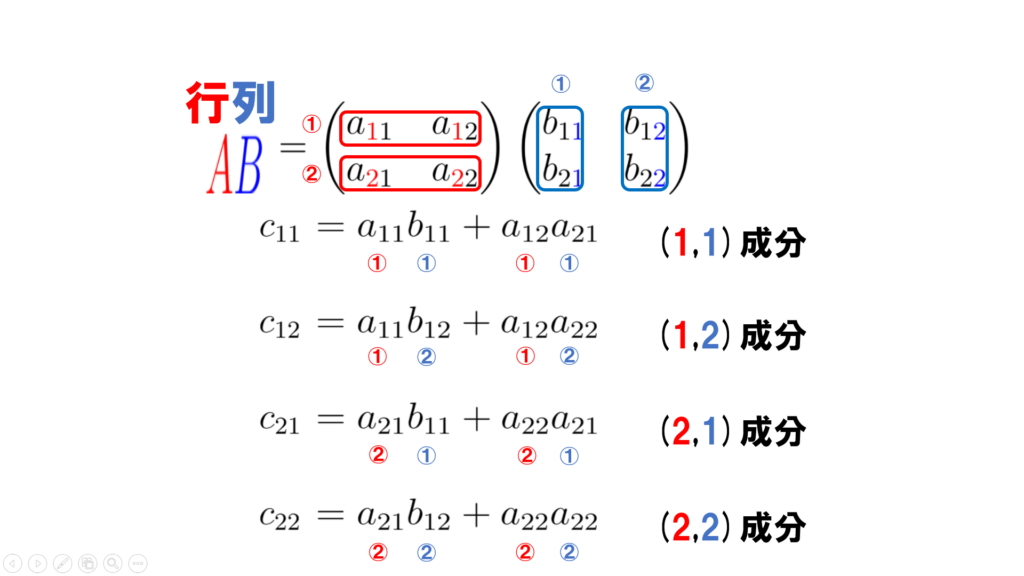
\includegraphics[height=0.8\textheight]{../resources/mat-mul}
  \end{figure}
\end{frame}

\begin{frame}{単純計算アルゴリズム}
  \begin{figure}
    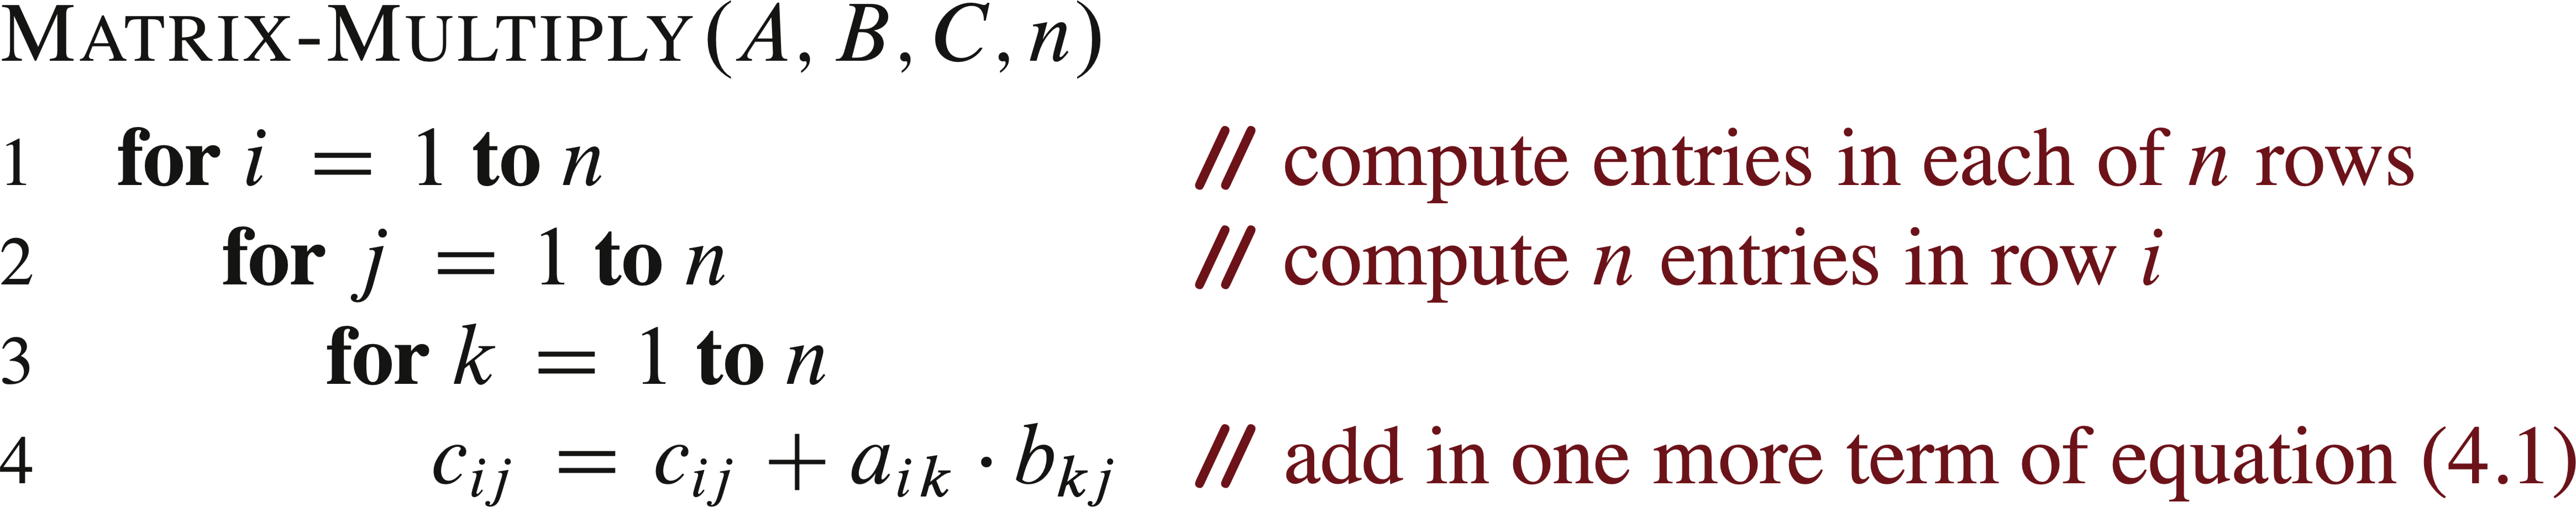
\includegraphics[width=0.95\textwidth]{../resources/pseudo-04-01}
  \end{figure}
\end{frame}

\note[itemize]{
  \item まず $c_{ij}$ を $0$ に初期化します。
  \item 最初の2つの for ループは積の各要素を繰り返します。
  \item 一番深い for ループは積の各要素を計算です。
}

\begin{frame}{単純な分割統治法}
  行列 $A$ と $B$ を4分割して、以下の計算をする
  \begin{align*}
    \begin{pmatrix}
      C_{11} & C_{12} \\
      C_{21} & C_{22}
    \end{pmatrix}
    & =
    \begin{pmatrix}
      A_{11} & A_{12} \\
      A_{21} & A_{22}
    \end{pmatrix}
    \begin{pmatrix}
      B_{11} & B_{12} \\
      B_{21} & B_{22}
    \end{pmatrix} \\
    & =
    \begin{pmatrix}
      A_{11} \cdot B_{11} + A_{12} \cdot B_{21} &
      A_{11} \cdot B_{12} + A_{12} \cdot B_{22} \\
      A_{21} \cdot B_{11} + A_{22} \cdot B_{21} &
      A_{21} \cdot B_{12} + A_{22} \cdot B_{22} 
    \end{pmatrix}
  \end{align*}
\end{frame}

\begin{frame}{単純な分割統治法のアルゴリズム}
  \begin{figure}
    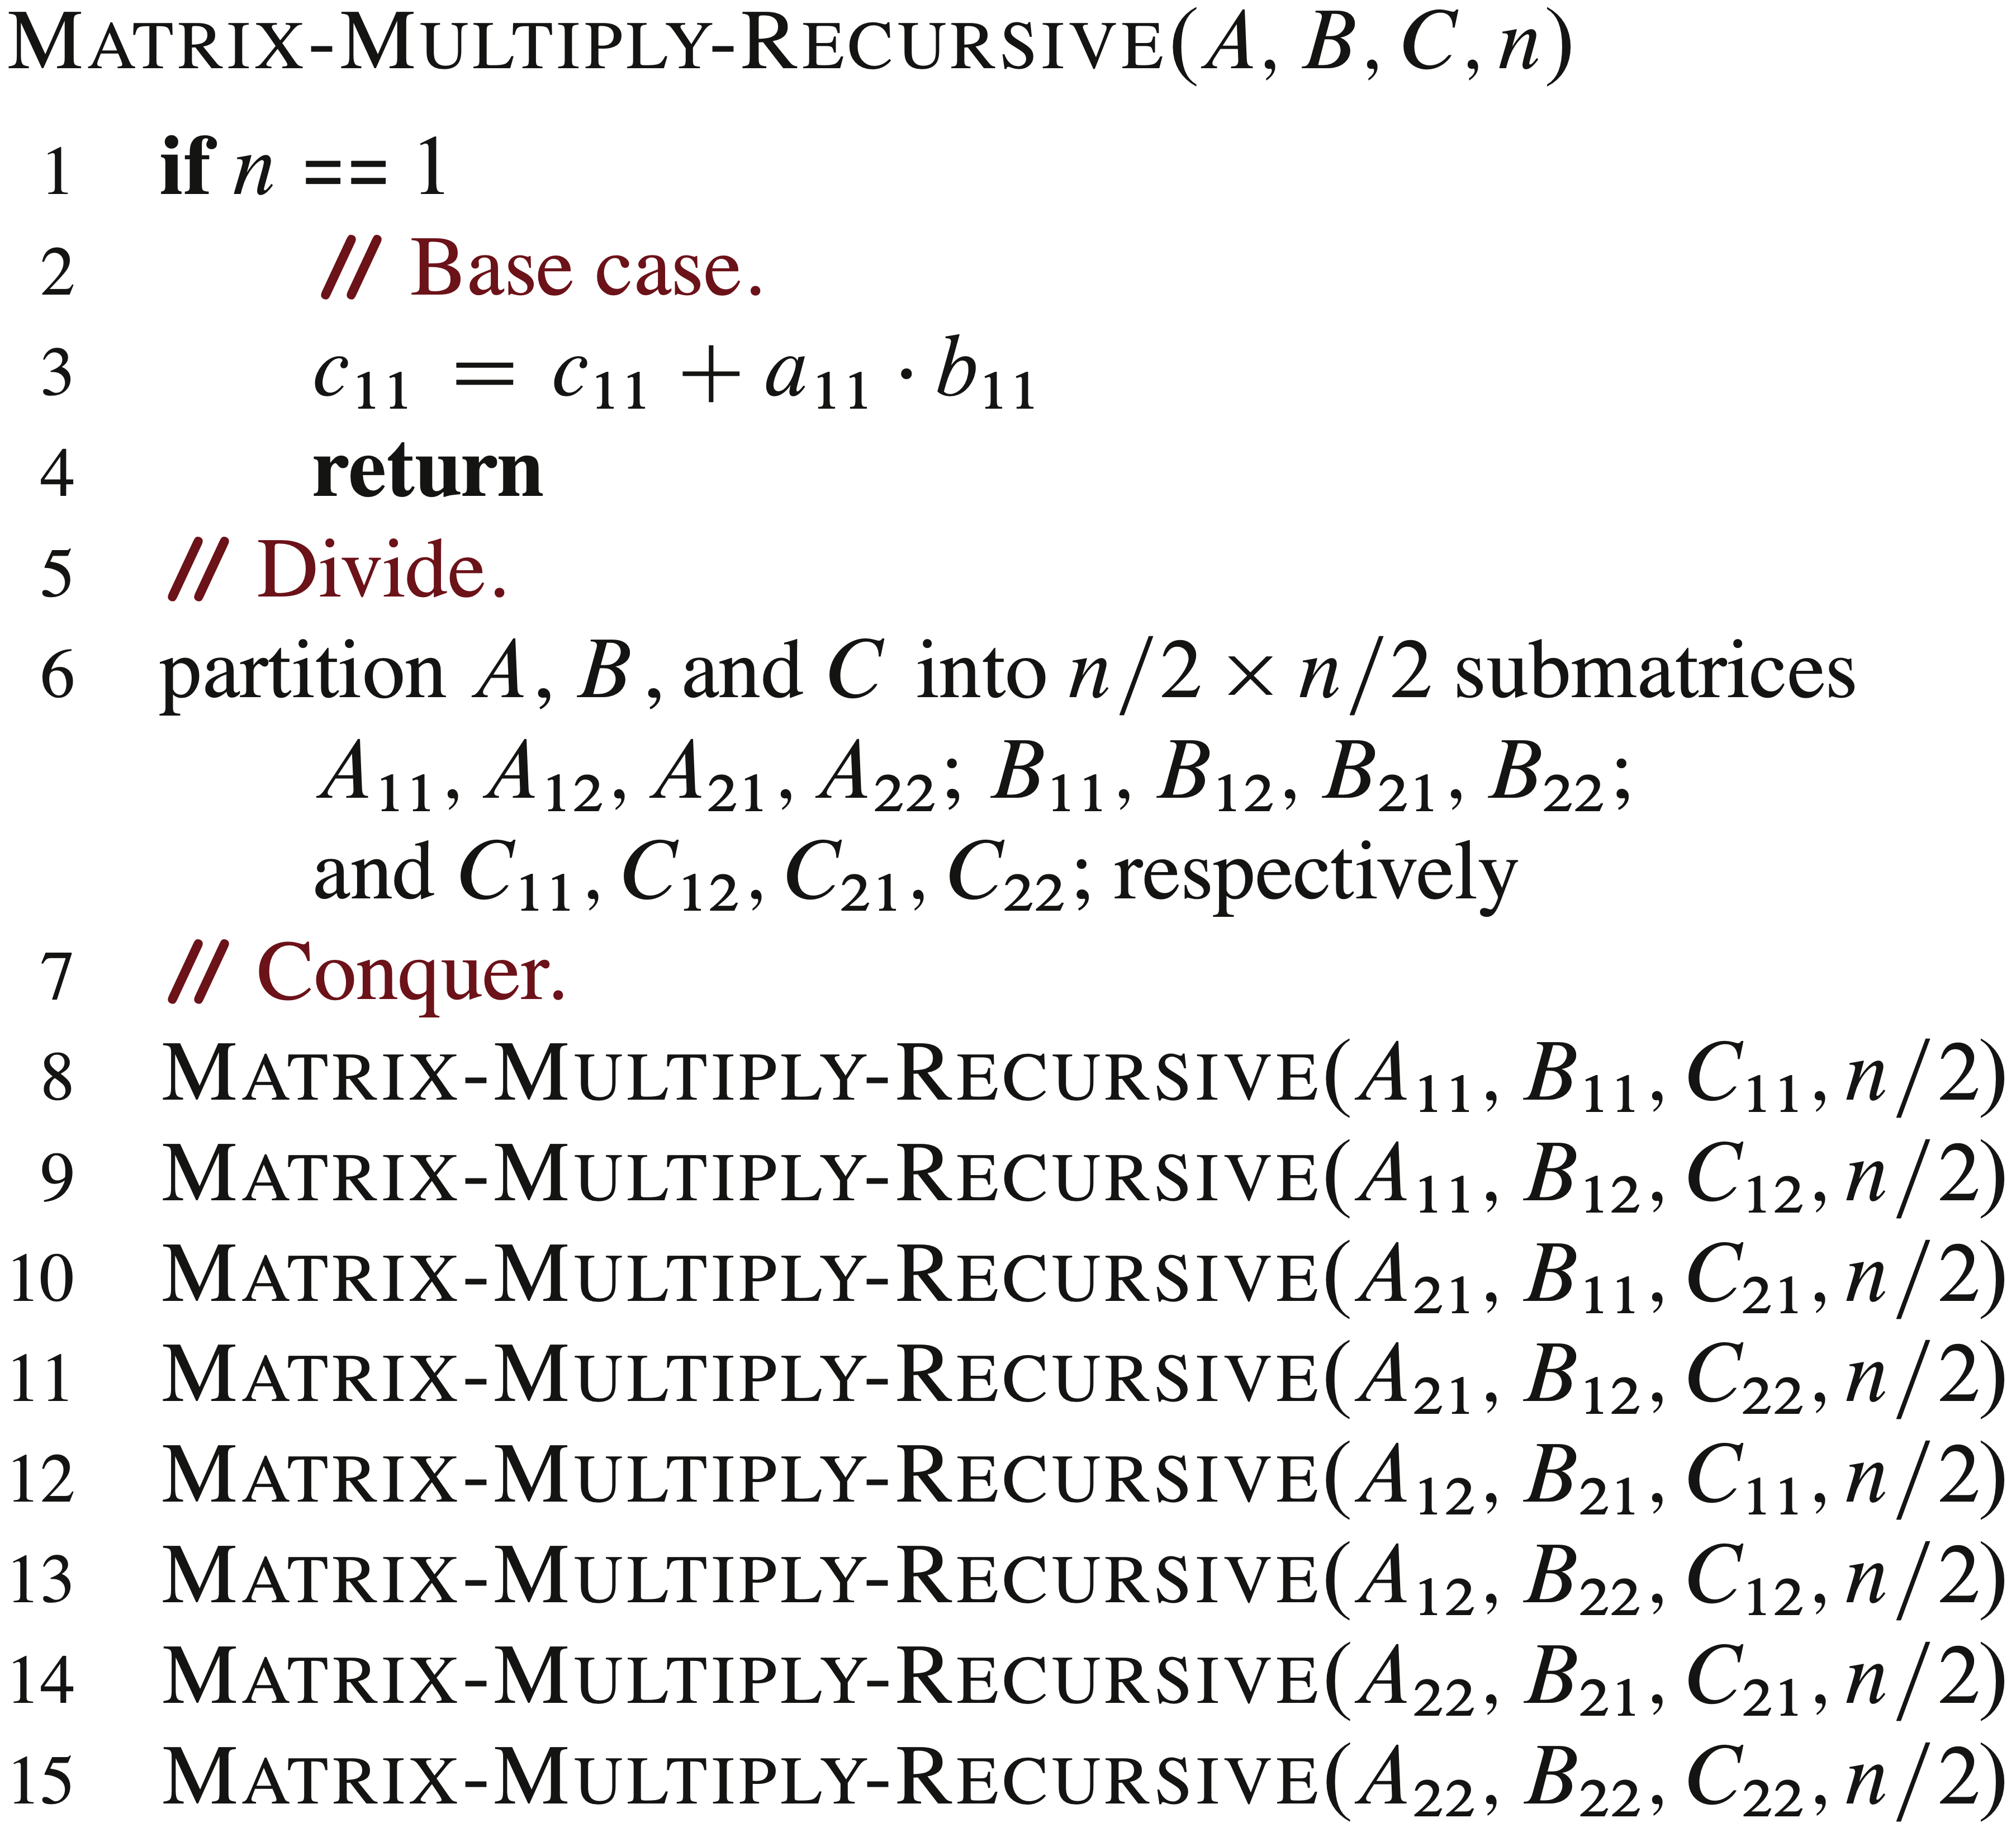
\includegraphics[height=0.60\textheight]{../resources/pseudo-04-02}
  \end{figure}
  実行時間は漸化式 $T(n) = 8T(n/2) + \Theta(1)$ になるが、
  この実行時間は $\Theta(n^3)$ である。
\end{frame}

\note[itemize]{
  \item 単純に分割しても計算量は変わりませんね。
}

\begin{frame}{Strassen のアルゴリズム}
  \begin{itemize}
    \item 詳細は各自確認してください。
    \item 要は実行時間は $T(n) = 7T(n/2) + \Theta(n^2) = \Theta(n^{2.81})$。
  \end{itemize}
\end{frame}

\note[itemize]{
  \item 詳細は細かいのでここで紹介しません。
  \item 実行時間の漸化式をどうやって解析するのが今回のキモです。
}

\section*{アルゴリズム的な漸化式の解く方法}

\begin{frame}
  \sectionpage{}
\end{frame}

\begin{frame}{漸化式を解く方法}
  \begin{itemize}
    \item \textbf{置き換え法(substitution method)}では、推測し数学的帰納法で証明する。
    \item \textbf{再帰木法(recursion-tree method)}では、漸化式を木と見立てて、各階層
    の総実行時間を計算し、全ての階層の総和を計算する。
    \item \textbf{マスター法(master method)}では、$a>0$ かつ $b>1$ のときの漸化式
    $T(n) = aT(n/b)+f(n)$ の閉じた限界式を求める。
    \item \textbf{Akra-Bazzi 法}では、分割統治の漸化式の閉じた限界式を一般的に求める。
  \end{itemize}
\end{frame}

\begin{frame}{置き換え法(substitution method)}
  \begin{itemize}
    \item 定数を変数のままにして、限界を推測する。
    \item 数学的帰納法を用いて限界の正しさを証明し、定数を特定する。
  \end{itemize}
\end{frame}

\begin{frame}{例}
  \begin{equation}\label{eq:rec}
    T(n)=2T(\lfloor n/2\rfloor)+\Theta(n)
  \end{equation}
  のとき、$T(n)=O(n\lg n)$ を証明したい。

  \vspace{5mm}

  すべての $n\geq n_0$ に対して $T(n)\leq cn\lg n$、と仮定する。
  これを\textbf{帰納仮定(inductive hypothesis)}と名付ける。
  
  ただし、定数 $c>0$ と $n_0>0$ は証明過程で求める。

  \vspace{5mm}

  これが証明できれば、$T(n)=O(n\lg n)$ も証明されることになる。
\end{frame}

\note[itemize]{
  \item 帰納仮定を証明したい。
}

\begin{frame}{例:数学的帰納法の帰納ケース(inductive case)}
  \begin{itemize}
    \item<+-> $[n_0,n)$ で $T(n)\leq cn\lg n$ が成り立つなら、$n$
    でも成り立つことを証明する。
    \item<+-> $n\geq 2n_0$ なら、$\lfloor n/2\rfloor$ で成り立つ。
    従って、$T(\lfloor n/2\rfloor)\leq c\lfloor n/2\rfloor\lg(\lfloor n/2\rfloor)$。
    \item<+-> (\ref{eq:rec})に代入すると、
    \begin{align*}
      T(n) & \leq 2(c\lfloor n/2\rfloor\lg(\lfloor n/2\rfloor)) + \Theta(n) \\
           & \leq 2(c(n/2)\lg(n/2)) + \Theta(n) \\
           & = cn\lg(n/2) + \Theta(n) \\
           & = cn\lg n - cn\lg 2 + \Theta(n) \\
           & = cn\lg n - cn + \Theta(n) \\
           & \leq cn\lg n
    \end{align*}
    \item<+-> これにより、$n\geq 2n_0$のとき成り立つことを証明した。
  \end{itemize}
\end{frame}

\note[itemize]{
  \item 帰納仮定の帰納ケースを証明する。
  \item 整数上の数学的帰納法の帰納ケースは「$n-1$までが成り立つなら$n$も成り立つ」
  を証明する。
  \item 帰納仮定に代入。
  \item 結果を漸化式に代入。
  \item 最後の行では $c$ の選び方によって、$cn$ が $\Theta(n)$ に隠されている
  無名の関数より大きくなるために不等式が成り立つ。
}

\begin{frame}{例:数学的帰納法の基底ケース(base case)}
  \begin{itemize}
    \item<+-> $n_0\leq n<2n_0$ のとき、$T(n)\leq cn\lg n$ が成り立つことを証明する。
    \item<+-> ここで $c$ と $n_0$ の条件も求める。
    \item<+-> $n_0>1$ の条件下 $\lg n>0$ よって $n\lg n>0$。
    \item<+-> $n_0=2$ と選ぶ。
    \item<+-> $T(n)$ はアルゴリズム的という前提の元で $T(2)$ と $T(3)$ が定数。
    \item<+-> $c=\max\{T(2), T(3)\}$ と選ぶ。
    \item<+-> よって、
    \begin{align*}
      T(2) \leq c & < (2\lg 2)c \\
      T(3) \leq c & < (3\lg 3)c
    \end{align*}
    基底ケースを証明することができた。
    \item<+-> 従って、すべての$n\geq 2$に対して、$T(n)\leq cn\lg n$ の証明ができた。
  \end{itemize}
\end{frame}

\note[itemize]{
  \item 帰納仮定の基底ケースを証明する。
  \item 帰納ケースでは、$n\geq 2n_0$の場合を証明したが、今度$n_0\leq n<2n_0$の場合を証明。
  \item アルゴリズム的というのは、必ず漸化式の基底ケースに帰着して、有限時間内に終了。
}

\begin{frame}{練習問題}
  手を動かして証明してみましょう!
  \begin{enumerate}
    \item $T(n)=T(n-1)+n$ の解は $T(n)=O(n^2)$
    \item $T(n)=T(n/2)+\Theta(1)$ の解は $T(n)=O(\lg n)$
    \item $T(n)=2T(n/2)+n$ の解は $T(n)=\Theta(n\lg n)$
    \item $T(n)=2T(n/2+17)+n$ の解は $T(n)=O(n\lg n)$
    \item $T(n)=2T(n/3)+\Theta(n)$ の解は $T(n)=\Theta(n)$
    \item $T(n)=4T(n/2)+\Theta(n)$ の解は $T(n)=\Theta(n^2)$
  \end{enumerate}
\end{frame}

\note[itemize]{
  \item ここでやりません。
  \item このスライドを後で見て、練習したい方はどうぞ。
}

\begin{frame}{再帰木法(recursion-tree method)}
  \begin{itemize}
    \item 漸化式を木と見立てて、各階層の総実行時間を計算し、全ての階層の総和を計算する。
    \item この方法で直接照明してもいいし、置き換え法の推測のために使ってもいい。
  \end{itemize}
\end{frame}

\begin{frame}{例}
  $T(n)=3T(n/4)+\Theta(n^2)$の上界を求めたい。
\end{frame}

\begin{frame}{例:図}
  \begin{figure}
    \includegraphics[height=0.85\textheight]{../resources/fig04.01}
  \end{figure}
\end{frame}

\note[itemize]{
  \item まず $T(n)$ を根にします。
  \item 次は $T$ で表されている葉っぱを再帰的に作ります。
  \item 節点を漸化式じゃないほうの項にして、この場合は $\Theta(n^2)$ なので、
  係数を $c$ にして、書きます。その子節点は部分問題にしていきます。
  \item 2-3回繰り返していって、基底ケースを書く。
  \item 分割統治法の基底ケースは「問題の大きさは特定な大きさより小さいとき直接な方法で解く」
  とあるため、実行時間は定数で $\Theta(1)$になります。
  \item 次は各層の実行時間の和を計算して、層の数を計算して、総和を取ります。
}

\begin{frame}{例:計算}
  \begin{align*}
    T(n) & = cn^2 + \frac{3}{16}cn^2 + \left(\frac{3}{16}\right)^2cn^2 + \cdots
             + \left(\frac{3}{16}\right)^{\log_4n}cn^2 + \Theta(n^{\log_43}) \\
         & = \sum_{i=0}^{\log_4n}\left(\frac{3}{16}\right)^icn^2
             + \Theta(n^{\log_43}) \\
         & < \sum_{i=0}^{\infty}\left(\frac{3}{16}\right)^icn^2
             + \Theta(n^{\log_43}) \\
         & = \frac{1}{1-(3/16)}cn^2+\Theta(n^{\log_43}) \\
         & = \frac{16}{13}cn^2+\Theta(n^{\log_43}) \\
         & = O(n^2)
  \end{align*}
\end{frame}

\note[itemize]{
  \item この場合の総和はこう計算できますね。
}

\begin{frame}{マスター法(master method)}
  \begin{itemize}
    \item $a>0$ かつ $b>1$ のときの漸化式 $T(n) = aT(n/b)+f(n)$ の閉じた限界式を求める。
    \item この漸化式は問題の大きさ $n$ を $a$ 個大きさ $n/b$ の部分問題に分割統治法を
    用いたアルゴリズムの実行時間を示す。$f(n)$ は分割と統合にかかるコストを表す。
  \end{itemize}
\end{frame}

\begin{frame}
  \begin{theorem}[マスター定理(master theorem)]
    $a>0$ と $b>1$ を定数として、$f(n)$ を十分に大きい実数に定義されかつ非負の関数とする。
    $n\in\mathbb{N}$ 上の漸化式 $T(n)$ をこのように定義する:
    \[
      T(n) = aT(n/b)+f(n)
    \]
    ただし $aT(n/b)$ は厳密に $a'T(\lfloor n/b\rfloor)+a''T(\lceil n/b\rceil)$
    であり、$a'\geq0$ かつ $a''\geq0$ かつ $a=a'+a''$である。このとき、$T(n)$の
    漸近的特徴は以下のように得られる。
    \begin{enumerate}
      \item $f(n)=O(n^{\log_ba-\epsilon})$となるような定数$\epsilon >0$が存在したら、
      $T(n)=\Theta(n^{\log_ba})$である。
      \item $f(n)=\Theta(n^{\log_ba}\lg^kn)$となるような定数$k\geq 0$が存在したら、
      $T(n)=\Theta(n^{\log_ba}\lg^{k+1}n)$である。
      \item $f(n)=\Omega(n^{\log_ba+\epsilon})$となるような定数$\epsilon >0$が存在し、
      しかもある定数 $c<1$ と十分に大きい $n$ に対して、$af(n/b)\leq cf(n)$ が成り立ったら、
      $T(n)=\Theta(f(n))$である。
    \end{enumerate}
  \end{theorem}
\end{frame}

\note[itemize]{
  \item 第一印象:こわい。
  \item 上の方は、このような漸化式で使えますよ、という定理の適応条件ですね。
  大体アルゴリズム解析で見る漸化式はこの形です。
  \item 次はこの3つの $f(n)$ の場合分けです。
  \item 1は $f(n)$ の上界がある条件に満たす場合。
  \item 2は $f(n)$ のタイトな限界がある条件に満たす場合。
  \item 3は $f(n)$ の下界がある条件に満たす場合。
  \item 全ての条件は $n^{\log_ba}$ に関連してる。
}

\begin{frame}{マスター定理を直感的に見てみよう}
  \begin{itemize}
    \item<+-> $aT(n/b)$ と $f(n)$ の再帰による増加率を比較する。
    \item<+-> $aT(n/b)$ の再帰による漸近的増加の限界は $O(n^{\log_ba})$ である。
    \item<+-> $n^{\log_ba}$ を\textbf{分水嶺関数(watershed function)}という。
    \item<+-> 1の場合は $aT(n/b)$ の増加率が大きい。
    \item<+-> 2の場合は同じぐらい。
    \item<+-> 3の場合は $f(n)$ の増加率が大きい。
    \item<+-> 1と3の場合でいう増加率の差は\textbf{多項式的な差}以上なければならない。
  \end{itemize}
\end{frame}

\note[itemize]{
  \item $aT(n/b)$ という項が再帰的に足し算していけば、どれぐらいの増加率があるのか?
  \item $f(n)$ という項が再帰的に足し算していけば、どれぐらいの増加率があるのか?
  \item この2つの増加率を比較して、場合分けしている。
  \item 前のスライドで全ての条件は $n^{\log_ba}$ に関連していると言いましたが、
  これは $aT(n/b)$ という項の再帰による漸近的増加率。
  \item これを名付けて、軸にして $f(n)$ という項の再帰による漸近的増加率と比較します。
  \item 1の場合は $aT(n/b)$ の増加率が大きいため、
  漸化式全体の漸近的限界は分水嶺関数のオーダになる。
  \item 2の場合は同じぐらいだから、漸化式全体の漸近的限界はそのコンビネーションです。
  \item 3の場合は $f(n)$ の増加率が大きいため、
  漸化式全体の漸近的限界は $f(n)$ のオーダになる。
}

\begin{frame}{マスター定理を使ってみる:マージソート}
  \begin{itemize}
    \item<+-> 漸化式は $T(n)=2T(n/2)+\Theta(n)$ である。
    \item<+-> $a=2$ と $b=2$、よって分水嶺関数は $n^{\log_22}=n$ である。
    \item<+-> $k=0$ とおき $f(n)=\Theta(n)=\Theta(n^{\log_ba}\lg^kn)$、よって2の場合になる。
    \item<+-> 従って、$T(n)=\Theta(n^{\log_ba}\lg^{k+1}n)=\Theta(n\lg n)$ である。
  \end{itemize}
\end{frame}

\note[itemize]{
  \item 分水嶺関数と $f(n)=\Theta(n)$ は同じオーダだから1と3の場合ではなさそう。
  \item じゃ、2の場合の $k$ を考えましょう。
}

\begin{frame}{マスター定理を使ってみる:行列積の単純分割統治}
  \begin{itemize}
    \item<+-> 漸化式は $T(n)=8T(n/2)+\Theta(1)$ である。
    \item<+-> $a=8$ と $b=2$、よって分水嶺関数は $n^{\log_28}=n^3$ である。
    \item<+-> 任意の正の $\epsilon<3$ をとれば $f(n)=O(n^{3-\epsilon})$ がなりたつ。
    \item<+-> 分水嶺関数 $n^3$ は $f(n)=\Theta(1)$ より、多項式的な増加率の差を持つ。
    よって1の場合になる。
    \item<+-> 従って、$T(n)=\Theta(n^3)$ である。
  \end{itemize}
\end{frame}

\note[itemize]{
  \item 分水嶺関数 $n^3$ と $f(n)=\Theta(1)$ とを比較して、
  次数が $3$ の差があるので、1の場合になります。
}

\begin{frame}{マスター定理を使ってみる:行列積の Strassen のアルゴリズム}
  \begin{itemize}
    \item<+-> 漸化式は $T(n)=7T(n/2)+\Theta(n^2)$ である。
    \item<+-> $a=7$ と $b=2$、よって分水嶺関数は $n^{\log_27}=n^{\lg 7}$。
    \item<+-> $\lg 7 > 2$ なので、任意の正の $\epsilon<\lg 7-2$ をとれば $f(n)=O(n^{\lg 7-\epsilon})$ がなりたつ。
    \item<+-> 分水嶺関数 $n^{\lg 7}$ は $f(n)=\Theta(n^2)$ より、多項式的な増加率の差を持つ。
    よって1の場合になる。
    \item<+-> 従って、$T(n)=\Theta(n^{\lg 7})$。
  \end{itemize}
\end{frame}

\note[itemize]{
  \item 分水嶺関数 $n^{2.81}$ と $f(n)=\Theta(n^2)$ とを比較して、
  次数が $0.8$ 以上の差があるので、1の場合になります。
}

\begin{frame}{飛ばす内容}
  \begin{itemize}
    \item マスター定理の証明
    \item Akra-Bazzi 法
  \end{itemize}
\end{frame}

\section*{確率的解析と乱択アルゴリズム}

\begin{frame}
  \sectionpage{}
\end{frame}

\begin{frame}{採用問題(hiring problem)}
  \begin{itemize}
    \item 採用エイジェントに依頼して、新しい助手を採用したい。
    \item 毎日候補を紹介してもらい、面接して、採用するかどうかを判断する。
    \item 面接するときに、エイジェントに少量の料金を払う。
    \item 採用するときに、解雇にかかるコストと大量の料金をエイジェントに払う。
    \item もっとも適した助手を雇いたい。
  \end{itemize}
\end{frame}

\begin{frame}{単純アルゴリズム}
  \begin{itemize}
    \item 面接した候補が現在の助手より適任なら採用する。
    \item どんな時点でも採用される候補は今までもっとも適任であることが保証される。
  \end{itemize}
  \begin{figure}
    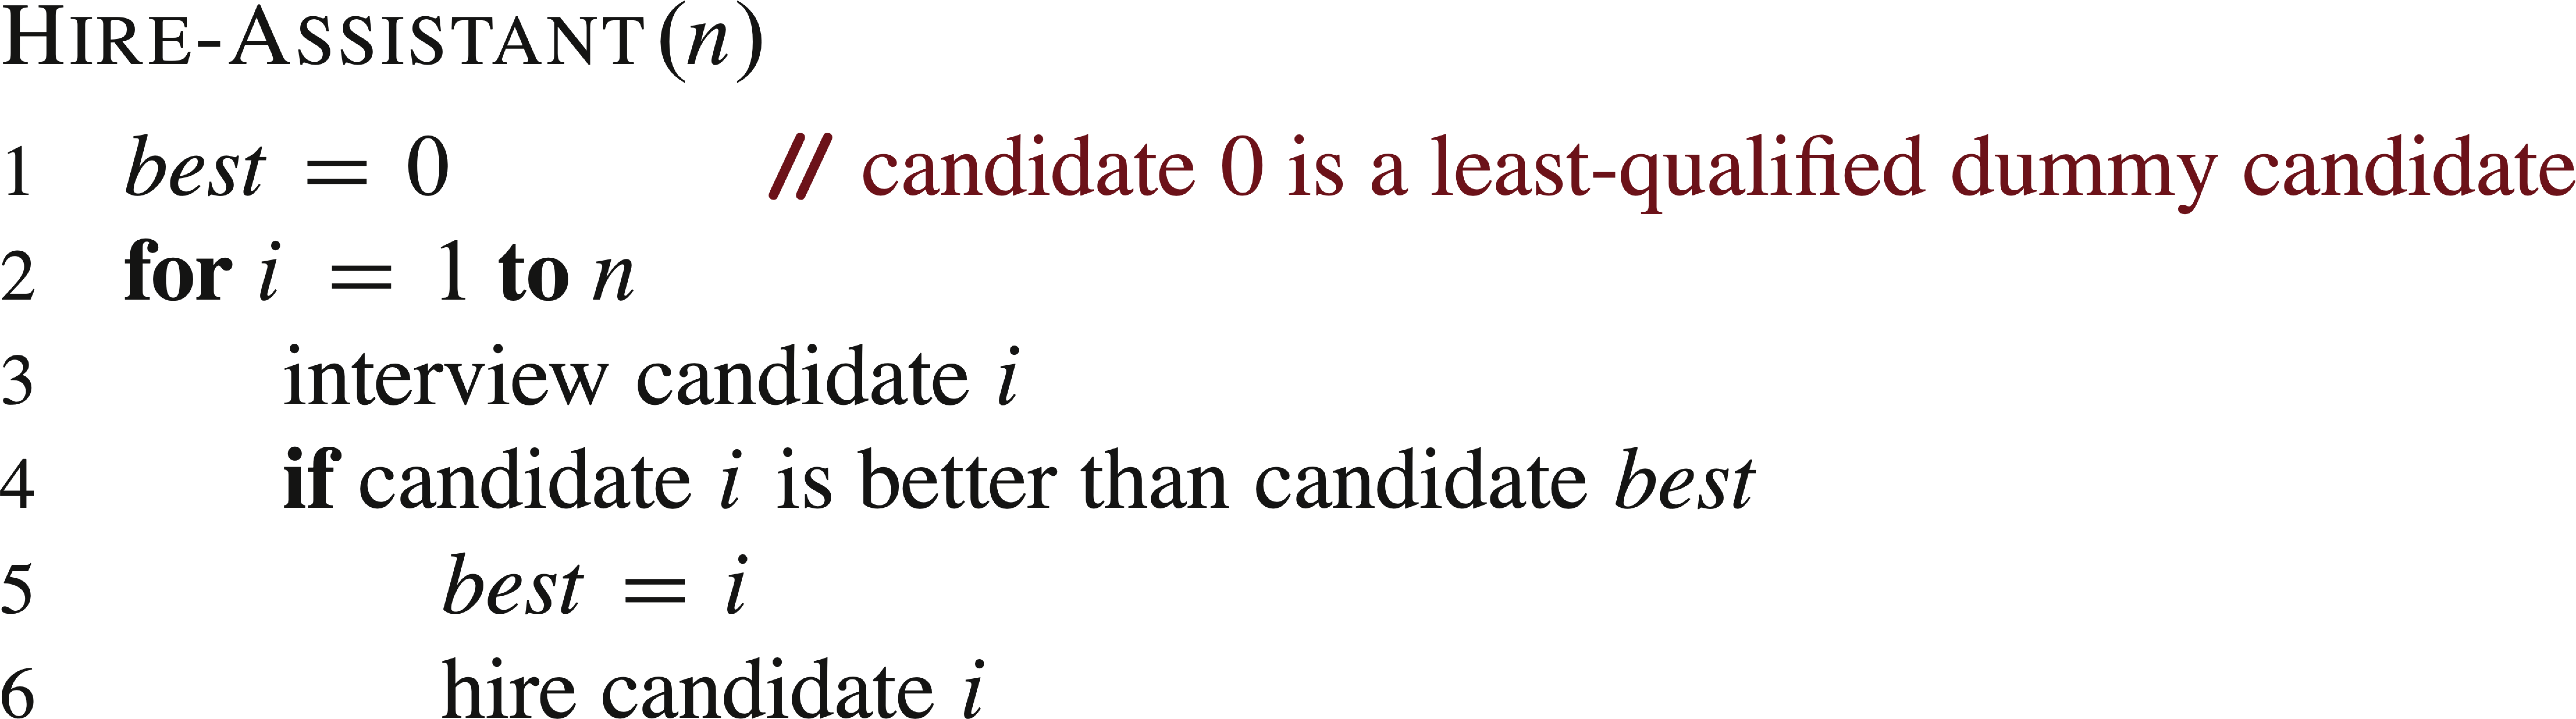
\includegraphics[width=0.90\textwidth]{../resources/pseudo-05-01}
  \end{figure}
\end{frame}

\begin{frame}{費用解析}
  \begin{itemize}
    \item<+-> 実行時間ではなく、費用を解析する。
    \item<+-> 面接のコスト(安い)を $c_i$ として、採用のコスト(高い)を $c_h$ とする。
    \item<+-> 総コストは $O(c_in+c_hm)$。
    \item<+-> 何人採用しても面接に関する費用は固定の $c_in$ であるので、
    採用のコスト $c_hm$ に着目する。
    \item<+-> 最悪時の解析:候補が適任でない順に紹介されるとき、一人ずつ全員採用することになる。
    コストは $O(c_hn)$ になる。
    \item<+-> ただし、どういう順番に紹介されるかわからないため、平均時を解析したい。
    \item<+-> 平均時解析するとき確率的解析を行う。
  \end{itemize}
\end{frame}

\begin{frame}{指標確率変数(indicator random variables)}
  \begin{itemize}
    \item<+-> 確率と期待値との間を行き来しやすいような方法。
    \item<+-> 標本空間 $S$ と事象 $A$ が与えられたとき、事象 $A$ に関する
    指標確率変数(indicator random variables) $I\{A\}$ をこのように定義する:
    \[
      I\{A\} =
      \begin{cases}
        1 & A \text{ が起きるとき} \\
        0 & A \text{ が起きないとき}
      \end{cases}
    \]
    \item<+-> $X_A = I\{A\}$ のとき $\E[X_A]=\Pr\{A\}$ である。
  \end{itemize}
\end{frame}

\begin{frame}{採用問題の解析}
  \begin{itemize}
    \item<+-> $X$ を新しい助手を採用する回数を表す確率変数とする。
    $\E[X]$ を求めたい。
    \item<+-> $X_i$ を候補 $i$ が採用される指標確率変数とする。つまり、
    \begin{align*}
      X_i & = I\{\text{候補 $i$ が採用される}\} \\
          & =
          \begin{cases}
            1 & \text{候補 $i$ が採用されるとき} \\
            0 & \text{候補 $i$ が採用されないとき} 
          \end{cases}
    \end{align*}
    \item<+-> よって、$X=X_1+X_2+\cdots+X_n$。
    \item<+-> そして、$\E[X_i]=\Pr\{\text{候補 $i$ が採用される}\}$。
    \item<+-> 候補 $i$ が候補 $1$ から $i-1$ より適任であるときのみ採用される。
    候補がランダムに判断されると仮定したため、
    候補 $i$ が候補 $1$ から $i-1$ より適任である確率は $1/i$ であり、以下が成り立つ:
    \[
      \E[X_i]=1/i
    \]
  \end{itemize}
\end{frame}

\begin{frame}{採用回数の期待値}
  $\E[X]$ を求める。
  \begin{align*}
    \E[X] & = \E\left[\sum_{i=1}^nX_i\right] \\
          & = \sum_{i=1}^n\E[X_i] \\
          & = \sum_{i=1}^n\frac{1}{i} \\
          & = \ln n + O(1)
  \end{align*}
  したがって、平均時の費用は $O(c_h\ln n)$ である。
  最悪時の $O(c_hn)$ より安い。
\end{frame}

\begin{frame}{乱択アルゴリズム}
  \begin{itemize}
    \item 候補が適任でない順に紹介される最悪の場合が起こらないようにしたい。
    \item 紹介される候補をランダムに選択する、
    \textbf{乱択アルゴリズム(randomized algorithm)}を採用。
    \item (確率的にみて)平均時の効率が保証される。
  \end{itemize}
  \begin{figure}
    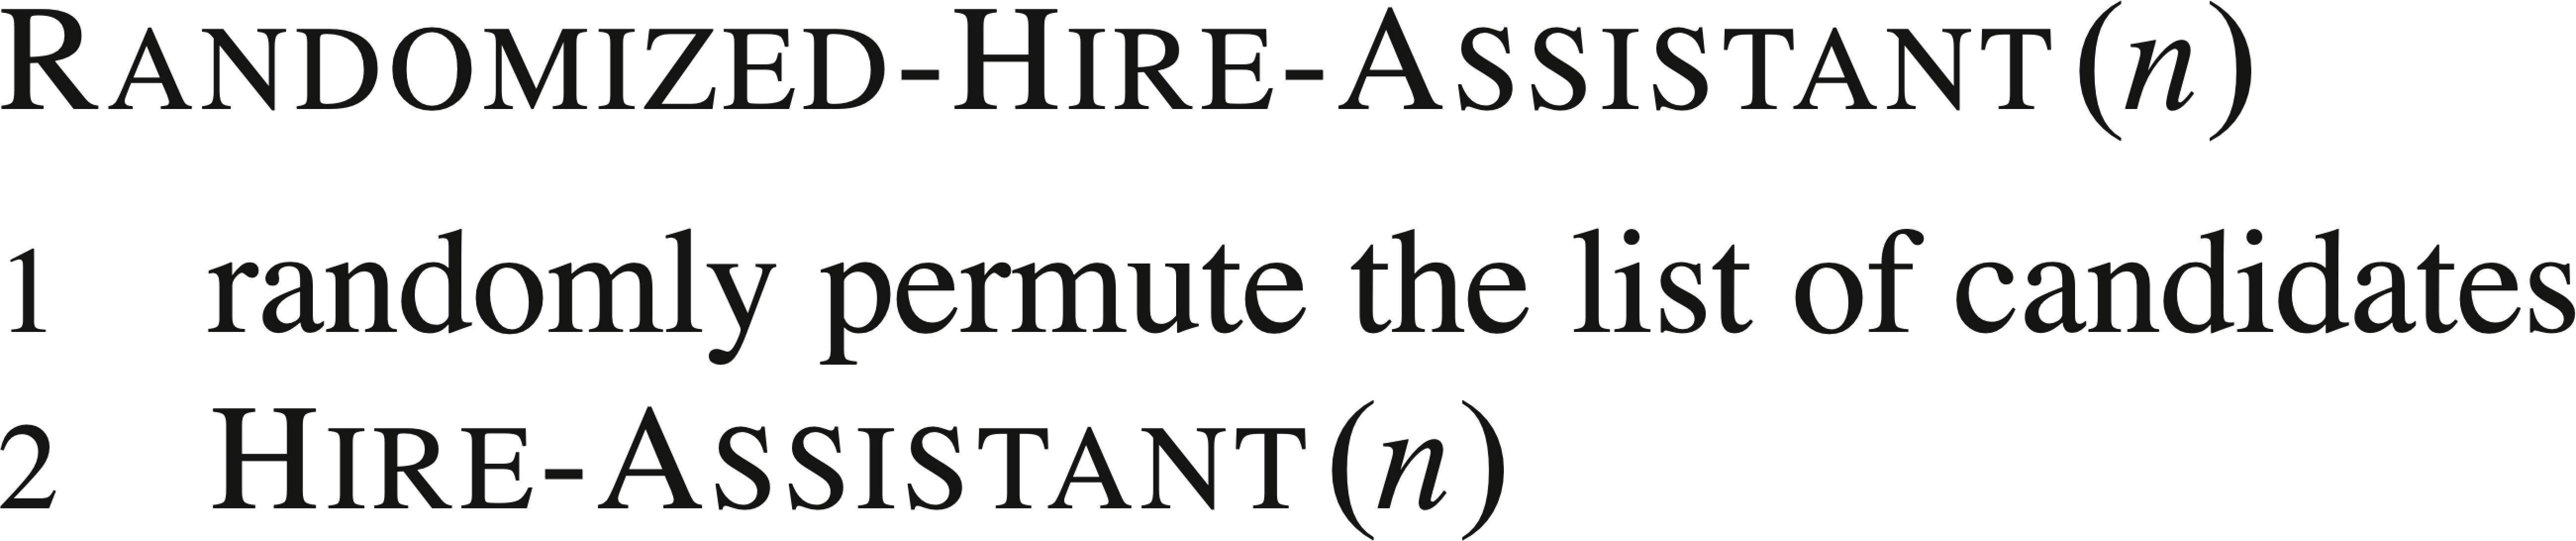
\includegraphics[width=0.70\textwidth]{../resources/pseudo-05-02}
  \end{figure}
\end{frame}

\end{document}
